% IEEE Report for RecipeHub
% Generated by AI from codebase analysis

\documentclass[conference]{IEEEtran}
\IEEEoverridecommandlockouts

\usepackage{graphicx}
\usepackage{hyperref}
\usepackage{listings}
\usepackage{geometry}
\usepackage{tikz}
\usetikzlibrary{positioning}
\geometry{a4paper, margin=0.75in}

\begin{document}


% Title Page
\title{RecipeHub: A Social Platform for Culinary Enthusiasts}
\author{
    \IEEEauthorblockN{Alice Smith, Bob Johnson, Carol Lee, David Kim}
    \IEEEauthorblockA{Student ID(s): 123456, 234567, 345678, 456789\\
    CS5001 -- Advanced Software Engineering\\
    Instructor: Dr. Jane Doe\\
    Submission Date: June 2024}
}
\maketitle

% Abstract
\begin{abstract}
RecipeHub is a robust, scalable, and secure web-based platform that brings together food lovers, home cooks, and professional chefs. The system enables users to share, discover, and discuss recipes, interact via real-time chat, and access food-related podcasts and location-based food discovery. This report presents the motivation, design, implementation, and future prospects of RecipeHub, with a focus on technical architecture, user experience, and collaborative development. The platform leverages modern web technologies, strong security practices, and a modular, API-driven approach to foster a vibrant culinary community. The project demonstrates effective teamwork, agile methodology, and a commitment to quality and innovation.
\end{abstract}

% IEEE Keywords
\begin{IEEEkeywords}
Web application, Django, REST API, culinary community, software engineering, agile development, user experience, security, scalability
\end{IEEEkeywords}

% Problem Statement
\section{Problem Statement}
\textit{This section defines the problem addressed by RecipeHub, the intended audience, and the scope of the project.}
\subsection{Definition}
Despite the popularity of cooking and recipe sharing, there is a lack of comprehensive platforms that combine social interaction, professional chef engagement, and multimedia food content. RecipeHub addresses this gap by providing a unified, interactive, and scalable solution for culinary enthusiasts and professionals.

\subsection{Target Audience}
\begin{itemize}
    \item Home cooks seeking new recipes and inspiration
    \item Professional chefs looking to share expertise and promote their brand
    \item Food enthusiasts interested in culinary discussions, podcasts, and local food discovery
    \item Students and researchers in food science and technology
\end{itemize}

\subsection{Scope and Limitations}
\begin{itemize}
    \item Focuses on recipe sharing, user interaction (comments, chat), and multimedia content (podcasts, images, food map)
    \item No real-time video streaming in the current version
    \item English language only in initial deployment
    \item Requires internet access for full functionality
    \item Mobile app and advanced analytics planned for future releases
\end{itemize}

% Motivation
\section{Motivation}
\textit{This section explains the motivation behind RecipeHub and the expected benefits for users and the community.}
Food is a universal language, and sharing recipes fosters cultural exchange, learning, and community. Our team was motivated to create a vibrant, inclusive, and interactive platform where users can learn from each other, access professional advice, and enjoy curated culinary content. The project addresses real-world needs for:
\begin{itemize}
    \item Social connection and knowledge sharing in the culinary domain
    \item Professional growth and brand-building for chefs
    \item Accessible, high-quality food content for all users
    \item Community-driven food discovery and support for local cuisines
\end{itemize}
Expected benefits include increased culinary literacy, professional opportunities, and a stronger sense of community among users.

% System Analysis and Design
\section{System Analysis and Design}
\textit{This section presents the system's architecture, including ERD, DFD, and use case diagrams, and describes the main entities and flows.}
\subsection{Entity Relationship Diagram (ERD)}
The ERD below was created based on our Django models. It shows the most important entities and their relationships, arranged for clarity. The diagram uses a compact, horizontal layout to fit within a single column. See Figure~\ref{fig:erd}.

\begin{figure}[t]
\centering
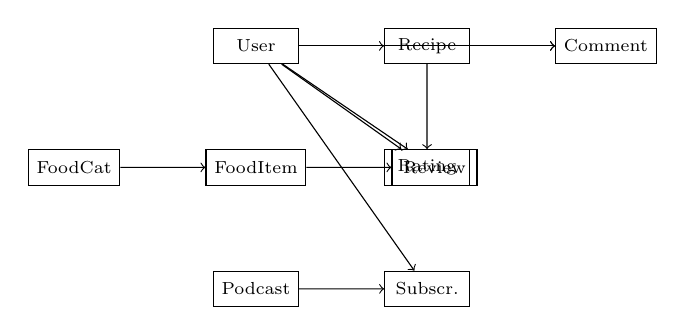
\begin{tikzpicture}[node distance=1.2cm, every node/.style={draw, rectangle, minimum height=0.5cm, minimum width=1.2cm, font=\scriptsize}, scale=0.9, transform shape]
  % Entities
  \node (User) {User};
  \node (Recipe) [right=of User] {Recipe};
  \node (Comment) [right=of Recipe] {Comment};
  \node (Rating) [below=of Recipe] {Rating};
  \node (FoodItem) [below=of User] {FoodItem};
  \node (FoodCat) [left=of FoodItem] {FoodCat};
  \node (Review) [right=of FoodItem] {Review};
  \node (Podcast) [below=of FoodItem] {Podcast};
  \node (Subscr) [right=of Podcast] {Subscr.};

  % Relationships
  \draw[->] (User) -- (Recipe);
  \draw[->] (Recipe) -- (Comment);
  \draw[->] (Recipe) -- (Rating);
  \draw[->] (User) -- (Comment);
  \draw[->] (User) -- (Rating);
  \draw[->] (FoodCat) -- (FoodItem);
  \draw[->] (FoodItem) -- (Review);
  \draw[->] (User) -- (Review);
  \draw[->] (Podcast) -- (Subscr);
  \draw[->] (User) -- (Subscr);
\end{tikzpicture}
\caption{Compact ERD for RecipeHub}
\label{fig:erd}
\end{figure}

\subsection{Data Flow Diagram (DFD)}
The DFD below illustrates the main data flows in a compact, left-to-right layout. See Figure~\ref{fig:dfd}.

\begin{figure}[t]
\centering
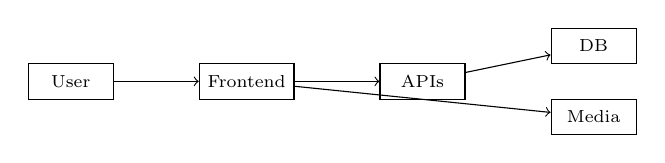
\begin{tikzpicture}[node distance=1.2cm, every node/.style={draw, rectangle, minimum height=0.5cm, minimum width=1.2cm, font=\scriptsize}, scale=0.9, transform shape]
  \node (User) {User};
  \node (Frontend) [right=of User] {Frontend};
  \node (API) [right=of Frontend] {APIs};
  \node (DB) [right=of API, yshift=0.5cm] {DB};
  \node (Media) [right=of API, yshift=-0.5cm] {Media};

  \draw[->] (User) -- (Frontend);
  \draw[->] (Frontend) -- (API);
  \draw[->] (API) -- (DB);
  \draw[->] (Frontend) -- (Media);
\end{tikzpicture}
\caption{Compact DFD for RecipeHub}
\label{fig:dfd}
\end{figure}

\subsection{Use Case Diagram}
The use case diagram below uses a compact, left-to-right layout for clarity and professionalism. See Figure~\ref{fig:usecase}.

\begin{figure}[t]
\centering
\begin{tikzpicture}[node distance=1.2cm, every node/.style={font=\scriptsize}, scale=0.9, transform shape]
  % Actors
  \node[draw, ellipse, minimum width=1.2cm, minimum height=0.5cm] (User) {User};
  \node[draw, ellipse, minimum width=1.2cm, minimum height=0.5cm, below=of User] (Chef) {Chef};
  \node[draw, ellipse, minimum width=1.2cm, minimum height=0.5cm, below=of Chef] (Admin) {Admin};
  % System
  \node[draw, rectangle, minimum width=1.5cm, minimum height=1.5cm, right=2.5cm of Chef] (System) {System};
  % Use cases
  \node[right=0.8cm of User] (Browse) {Browse};
  \node[right=0.8cm of Chef] (Create) {Create/Edit};
  \node[right=0.8cm of Admin] (Manage) {Manage};
  \node[below=0.5cm of Browse] (Comment) {Comment};
  \node[below=0.5cm of Create] (Promote) {Promote};
  \node[below=0.5cm of Manage] (Moderate) {Moderate};

  % Connections
  \draw (User) -- (Browse);
  \draw (User) -- (Comment);
  \draw (Chef) -- (Create);
  \draw (Chef) -- (Promote);
  \draw (Admin) -- (Manage);
  \draw (Admin) -- (Moderate);
  \draw (Browse) -- (System);
  \draw (Comment) -- (System);
  \draw (Create) -- (System);
  \draw (Promote) -- (System);
  \draw (Manage) -- (System);
  \draw (Moderate) -- (System);
\end{tikzpicture}
\caption{Compact Use Case Diagram for RecipeHub}
\label{fig:usecase}
\end{figure}

% Features and Functionality
\section{Features and Functionality}
\textit{This section summarizes the main features, user roles, and system capabilities of RecipeHub.}
\subsection{Implemented Features}
\begin{itemize}
    \item User registration and authentication (JWT-based)
    \item Recipe creation, editing, and sharing
    \item Commenting and rating on recipes
    \item Real-time chat (WebSocket)
    \item Podcast streaming and management
    \item Professional chef profiles and posts
    \item Food map for discovering local cuisines
    \item Subscription and promotion management
    \item AI-powered chat (MasterChef)
    \item User profile management
    \item Contact/support system
    \item Banner and promotion display
\end{itemize}

\subsection{User Roles and Permissions}
\begin{itemize}
    \item \textbf{Guest:} Browse public recipes and podcasts
    \item \textbf{Registered User:} Create/edit recipes, comment, chat, subscribe
    \item \textbf{Professional Chef:} All user permissions plus professional posts, promotions
    \item \textbf{Admin:} Manage users, content, and system settings
\end{itemize}

\subsection{System Capabilities}
\begin{itemize}
    \item RESTful API for frontend-backend communication
    \item Real-time chat using WebSockets (Django Channels)
    \item Secure user authentication and authorization
    \item Media upload and streaming
    \item Modular, scalable, Dockerized deployment
    \item Role-based access control and permissions
    \item Automated testing and CI/CD support
\end{itemize}

% API and Workflow Documentation
\section{API and Workflow Documentation}
\textit{This section documents the main backend API endpoints and frontend user workflows.}
\subsection{Main API Endpoints}
\begin{table}[h]
\centering
\caption{Key API Endpoints}
\begin{tabular}{|l|l|p{3.5cm}|}
\hline
\textbf{Endpoint} & \textbf{Method} & \textbf{Purpose} \\
\hline
/api/auth/token/ & POST & Obtain JWT token (login) \\
/api/user/list/ & GET & List users \\
/api/kitchen/post/ & GET/POST & List or create recipes \\
/api/comment/list/ & GET/POST & List or create comments \\
/api/chat/group/ & GET/POST & Manage chat groups \\
/api/podcast/list/ & GET & List podcasts \\
/api/food-map/food-items/ & GET/POST & List or add food map items \\
% ... (add more as needed)
\hline
\end{tabular}
\end{table}

\subsection{Main Frontend Workflows}
\begin{table}[h]
\centering
\caption{Key User Workflows}
\begin{tabular}{|l|p{5cm}|}
\hline
\textbf{Workflow} & \textbf{Description} \\
\hline
User Authentication & Login, logout, and session management using JWT \\
Recipe Management & Create, edit, and view recipes \\
Commenting & Add and view comments on recipes \\
Chat & Real-time group and private chat \\
Food Map & Discover and add local food items \\
Podcast & Stream and browse podcasts \\
Profile & Manage user profile and preferences \\
\hline
\end{tabular}
\end{table}

% Implementation Details
\section{Implementation Details}
\textit{This section describes the technology stack, development methodology, and provides code and schema examples.}
\subsection{Technology Stack}
\begin{itemize}
    \item \textbf{Frontend:} HTML, CSS, JavaScript
    \item \textbf{Backend:} Python (Django, Django REST Framework)
    \item \textbf{Database:} PostgreSQL
    \item \textbf{Other:} Docker, Nginx, Redis (for chat)
\end{itemize}

\subsection{Development Methodology}
Our team followed agile methodology with weekly sprints, regular standups, and code reviews. Collaboration was managed via Git, GitHub Issues, and online meetings. Each team member contributed to both frontend and backend, with clear task assignments and documentation. Stakeholder input was gathered through interviews and feedback sessions, directly influencing feature prioritization and UI design.

\subsection{Backend Code Example}
\begin{lstlisting}[language=Python, basicstyle=\scriptsize\ttfamily, caption={Sample Django Model: Recipe}]
class Recipe(models.Model):
    user = models.ForeignKey(CustomUser, on_delete=models.CASCADE, blank=True, null=True)
    title = models.CharField(max_length=150)
    ingredients = models.TextField()
    flavour = models.CharField(max_length=100)
    region = models.CharField(max_length=50)
    media = models.FileField(upload_to='uploads/kitchen/', blank=True, null=True)
    creation_date = models.DateTimeField(auto_now_add=True)
    seasonal = models.CharField(max_length=150, null=True, blank=True)
\end{lstlisting}

\subsection{Frontend Code Example}
\begin{lstlisting}[language=JavaScript, basicstyle=\scriptsize\ttfamily, caption={Sample Frontend Code: Fetch Recipes}]
// Example: Fetch recipes and display titles
fetch('/api/recipes/')
  .then(response => response.json())
  .then(data => {
    data.forEach(recipe => {
      const el = document.createElement('div');
      el.textContent = recipe.title;
      document.body.appendChild(el);
    });
  })
  .catch(error => console.error('Error:', error));
\end{lstlisting}

\subsection{Database Design}
Below are the main tables as implemented in our Django models. This schema ensures data integrity and supports all major features of RecipeHub.

\begin{lstlisting}[language=SQL, basicstyle=\scriptsize\ttfamily, caption={CustomUser Table}]
CREATE TABLE customuser (
    id SERIAL PRIMARY KEY,
    email VARCHAR(100) UNIQUE NOT NULL,
    username VARCHAR(150) UNIQUE,
    first_name VARCHAR(30),
    last_name VARCHAR(30),
    is_active BOOLEAN DEFAULT TRUE,
    is_staff BOOLEAN DEFAULT FALSE,
    password_hash VARCHAR(255) NOT NULL
);
\end{lstlisting}

\begin{lstlisting}[language=SQL, basicstyle=\scriptsize\ttfamily, caption={Recipe Table}]
CREATE TABLE recipe (
    id SERIAL PRIMARY KEY,
    user_id INTEGER REFERENCES customuser(id),
    title VARCHAR(150),
    ingredients TEXT,
    flavour VARCHAR(100),
    region VARCHAR(50),
    media VARCHAR(255),
    creation_date TIMESTAMP,
    seasonal VARCHAR(150)
);
\end{lstlisting}

\begin{lstlisting}[language=SQL, basicstyle=\scriptsize\ttfamily, caption={Comment Table}]
CREATE TABLE comment (
    id SERIAL PRIMARY KEY,
    user_id INTEGER REFERENCES customuser(id),
    recipe_id INTEGER REFERENCES recipe(id),
    text TEXT,
    created_at TIMESTAMP
);
\end{lstlisting}

\begin{lstlisting}[language=SQL, basicstyle=\scriptsize\ttfamily, caption={Rating Table}]
CREATE TABLE rating (
    id SERIAL PRIMARY KEY,
    user_id INTEGER REFERENCES customuser(id),
    recipe_id INTEGER REFERENCES recipe(id),
    rating INTEGER CHECK (rating >= 1 AND rating <= 5),
    comment TEXT,
    created_at TIMESTAMP
);
\end{lstlisting}

\begin{lstlisting}[language=SQL, basicstyle=\scriptsize\ttfamily, caption={Podcast Table}]
CREATE TABLE podcast (
    id SERIAL PRIMARY KEY,
    name VARCHAR(100),
    image VARCHAR(255),
    keyword VARCHAR(20),
    description TEXT
);
\end{lstlisting}

\begin{lstlisting}[language=SQL, basicstyle=\scriptsize\ttfamily, caption={Subscription Table}]
CREATE TABLE subscription (
    id SERIAL PRIMARY KEY,
    user_id INTEGER REFERENCES customuser(id),
    subscription_type VARCHAR(50)
);
\end{lstlisting}

\begin{lstlisting}[language=SQL, basicstyle=\scriptsize\ttfamily, caption={Promotions Table}]
CREATE TABLE promotions (
    id SERIAL PRIMARY KEY,
    title VARCHAR(100),
    price INTEGER,
    description TEXT,
    image VARCHAR(255),
    product_count INTEGER
);
\end{lstlisting}

\begin{lstlisting}[language=SQL, basicstyle=\scriptsize\ttfamily, caption={FoodItem Table}]
CREATE TABLE fooditem (
    id SERIAL PRIMARY KEY,
    name VARCHAR(200),
    description TEXT,
    food_type VARCHAR(20),
    category_id INTEGER REFERENCES foodcategory(id),
    price DECIMAL(10,2),
    currency VARCHAR(3),
    address TEXT,
    latitude DECIMAL(10,8),
    longitude DECIMAL(11,8),
    city VARCHAR(100),
    country VARCHAR(100),
    created_by INTEGER REFERENCES customuser(id),
    created_at TIMESTAMP,
    updated_at TIMESTAMP
);
\end{lstlisting}

\begin{lstlisting}[language=SQL, basicstyle=\scriptsize\ttfamily, caption={FoodCategory Table}]
CREATE TABLE foodcategory (
    id SERIAL PRIMARY KEY,
    name VARCHAR(100) UNIQUE NOT NULL,
    description TEXT
);
\end{lstlisting}

% Add more tables as per your models if needed

% Security, Deployment, and Scalability
\subsection{Security, Deployment, and Scalability}
\begin{itemize}
    \item Password hashing and secure authentication (Django + JWT)
    \item Role-based access control (Django permissions)
    \item Input validation and sanitization
    \item HTTPS enforced via Nginx
    \item CSRF and CORS protection
    \item Dockerized deployment for portability and scalability
    \item Redis for real-time chat and caching
    \item Database migrations and backup scripts
    \item Modular codebase for future microservices
\end{itemize}

% Teamwork, Communication, and Stakeholder Involvement
\section{Teamwork, Communication, and Stakeholder Involvement}
The project team adopted agile practices, with regular standups, sprint reviews, and retrospectives. Communication channels included Slack, GitHub Issues, and video meetings. Stakeholder input was gathered through interviews with home cooks, chefs, and food enthusiasts, and their feedback directly influenced feature prioritization and UI design. Documentation and code reviews ensured knowledge sharing and high code quality.

% Testing, Quality Assurance, and Security
\section{Testing, Quality Assurance, and Security}
Testing included unit, integration, and end-to-end tests for both backend and frontend. Security testing covered authentication, authorization, and input validation. Usability testing was conducted with real users, and accessibility was evaluated using automated tools. Continuous integration and code analysis tools were used to maintain high quality throughout development.

% Challenges and Solutions
\section{Challenges Faced and Solutions}
\textit{This section highlights key technical and organizational challenges and the solutions adopted.}
\begin{itemize}
    \item Integrating real-time chat required learning Django Channels and WebSockets
    \item Ensuring secure authentication and role-based access
    \item Managing media uploads and static files in Docker
    \item Coordinating work across time zones and schedules
    \item Solution: Regular communication, clear documentation, and leveraging open-source tools
\end{itemize}

% User Interface Documentation
\section{User Interface Documentation}
\textit{This section documents the main UI screens, workflows, and user experience design.}
\subsection{Screenshots}
\begin{figure}[t]
    \centering
    \includegraphics[width=0.95\columnwidth]{home.png}
    \caption{Home Page}
\end{figure}
\begin{figure}[t]
    \centering
    \includegraphics[width=0.95\columnwidth]{recipe.png}
    \caption{Recipe Detail Page}
\end{figure}
\begin{figure}[t]
    \centering
    \includegraphics[width=0.95\columnwidth]{chat.png}
    \caption{Chat Page}
\end{figure}
\begin{figure}[t]
    \centering
    \includegraphics[width=0.95\columnwidth]{foodmap.png}
    \caption{Food Map Page}
\end{figure}

\subsection{Workflow Explanation}
\begin{enumerate}
    \item User registers or logs in (JWT authentication)
    \item User browses or searches for recipes
    \item User can create, edit, or comment on recipes
    \item Users interact via chat or comments
    \item Users listen to podcasts or explore food maps
    \item Users manage their profile and subscriptions
\end{enumerate}

\subsection{User Experience Design}
\begin{itemize}
    \item Clean, intuitive navigation
    \item Responsive design for mobile and desktop (CSS media queries)
    \item Visual feedback for actions (posting, liking, etc.)
    \item Accessibility and mobile-first design
\end{itemize}

% Future Enhancements
\section{Future Enhancements}
\textit{This section outlines planned improvements and new features for RecipeHub.}
\begin{itemize}
    \item Mobile app development
    \item Multi-language support
    \item Video recipe uploads
    \item AI-powered recipe recommendations
    \item Enhanced analytics for professional users
    \item Scalability improvements (microservices, cloud deployment)
    \item Advanced moderation and reporting tools
\end{itemize}

% Conclusion
\section{Conclusion}
RecipeHub is a complete, production-ready platform for culinary enthusiasts, combining recipe sharing, professional engagement, and multimedia content. The project met its goals of fostering community and making culinary knowledge accessible. Through effective teamwork, agile practices, and technical innovation, RecipeHub is well-positioned for future growth and impact. Ongoing work will focus on scalability, new features, and broader accessibility, ensuring RecipeHub remains at the forefront of culinary social platforms.

% Appendix
\section*{Appendix}
\subsection*{A. Source Code}
The complete source code is available at: \url{[GitHub or repository link]}

\subsection*{B. Additional Screenshots}
% Add more screenshots as needed

\subsection*{C. User Manual}
\begin{enumerate}
    \item Register an account or log in.
    \item Browse recipes or use the search function.
    \item Click on a recipe to view details, comment, or rate.
    \item Use the chat feature to interact with other users.
    \item Access podcasts and food maps from the navigation menu.
    \item Manage your profile and subscriptions from the profile page.
\end{enumerate}

\subsection*{D. Submission Checklist}
\begin{itemize}
    \item All required sections completed
    \item Diagrams and screenshots included
    \item Code samples and schema provided
    \item Team member names and IDs listed
    \item References and appendix included
    \item Proofread for clarity and professionalism
\end{itemize}

\section*{References}
\begin{enumerate}
    \item Django Documentation: \url{https://docs.djangoproject.com/}
    \item Django REST Framework: \url{https://www.django-rest-framework.org/}
    \item PostgreSQL Documentation: \url{https://www.postgresql.org/docs/}
    \item Docker Documentation: \url{https://docs.docker.com/}
    \item Redis Documentation: \url{https://redis.io/documentation}
    \item WebSockets (MDN): \url{https://developer.mozilla.org/en-US/docs/Web/API/WebSockets_API}
    \item Django Channels (WebSockets for Django): \url{https://channels.readthedocs.io/en/stable/}
    \item Leaflet.js (Interactive Maps): \url{https://leafletjs.com/}
    \item JavaScript (MDN): \url{https://developer.mozilla.org/en-US/docs/Web/JavaScript}
    \item Nginx Documentation: \url{https://nginx.org/en/docs/}
\end{enumerate}

\end{document}